\section{Wavelet-based results and comparison with baseline diffusion}

The wavelet cascade is assessed in two distinct settings. In the
\emph{reference-coarse} diagnostic, the $cA^2$ coefficient is taken from a
validation field and only the detail sub-bands are synthesized. This is not an
unconditional generation experiment: it isolates the quality of the
conditional detail models. In the \emph{generated-coarse} setting, the
initial $cA^2$ is itself sampled by a diffusion model, so that errors can
propagate through the full cascade.

The visual comparison in Figure~\ref{fig:ch5_wsgm_field_comparison} contrasts
the direct SGM baseline with the two wavelet-based settings at the same nominal
number of reverse steps. The reference-coarse WSGM samples are expected to be
the cleanest diagnostic of the detail models, whereas the generated-coarse
case measures the full unconditional cascade.

\begin{figure}[H]
    \centering

    \begin{subfigure}[c]{0.32\textwidth}
        \centering
        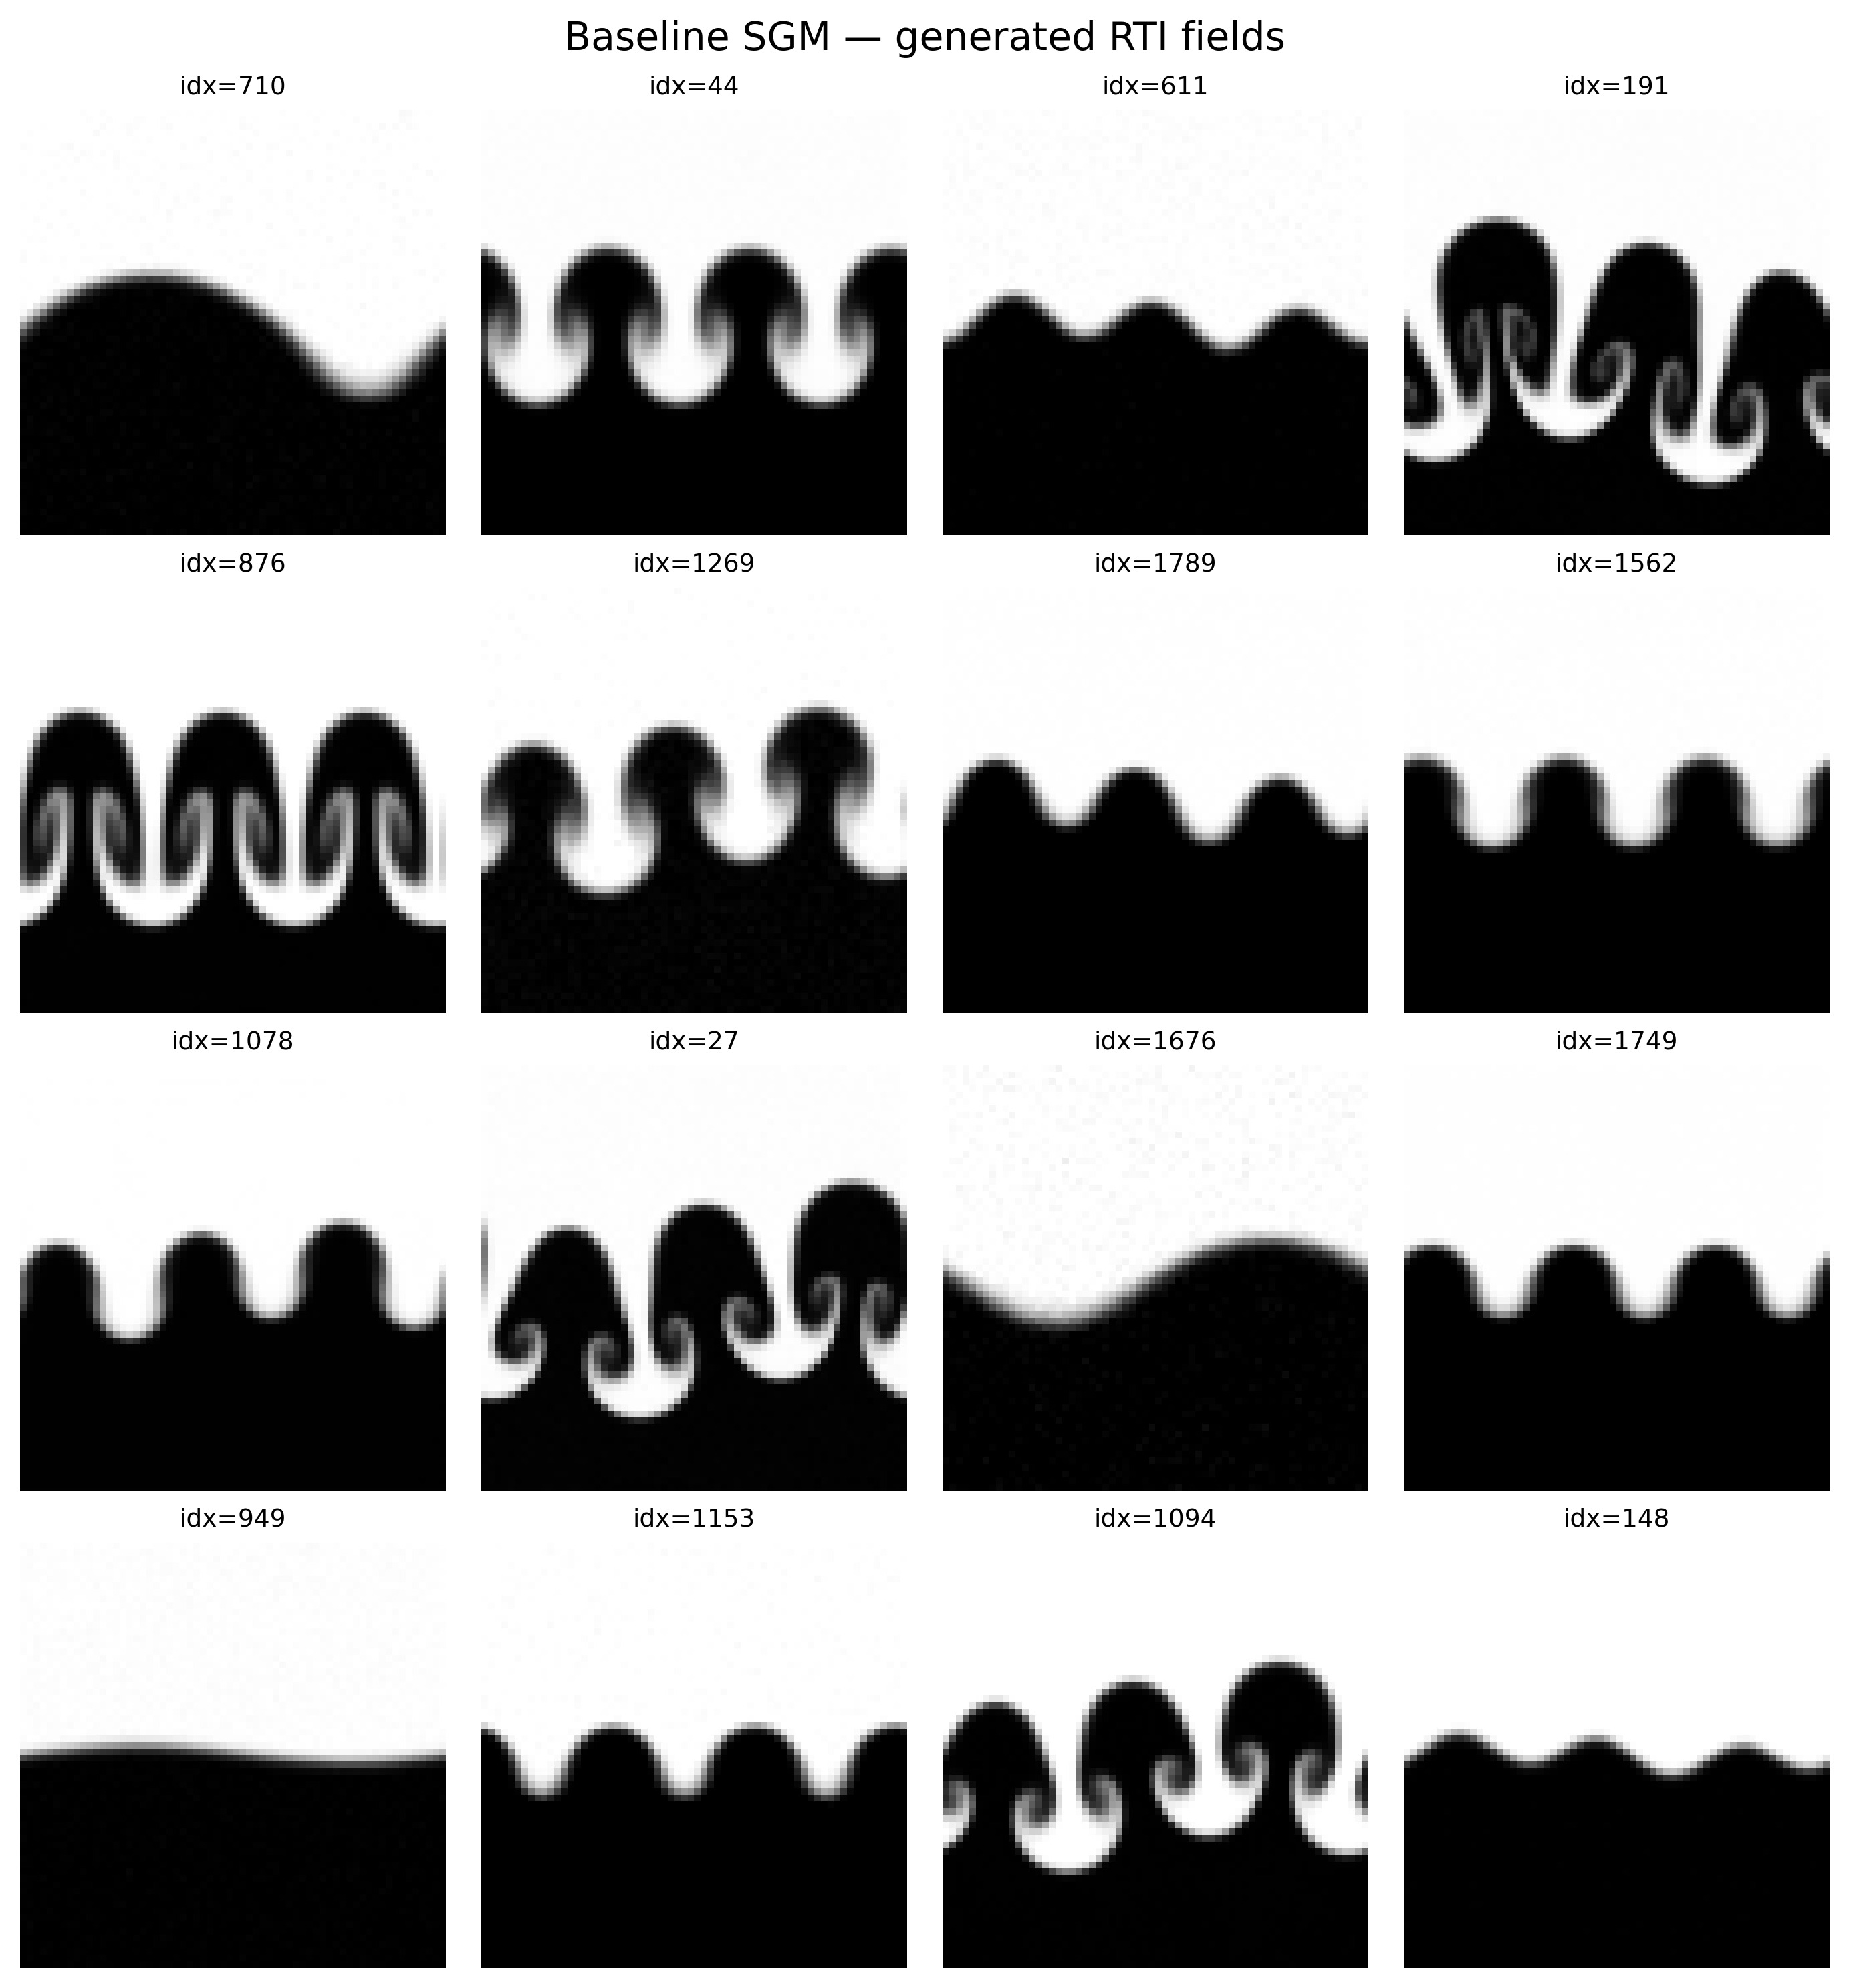
\includegraphics[
            width=\textwidth,
            height=\textwidth
        ]{figures/ch5/baseline_sgm_grid.png}
        \caption{SGM baseline with $128$ reverse steps.}
        \label{fig:ch5_wsgm_baseline_grid}
    \end{subfigure}
    \hfill
    \begin{subfigure}[c]{0.32\textwidth}
        \centering
        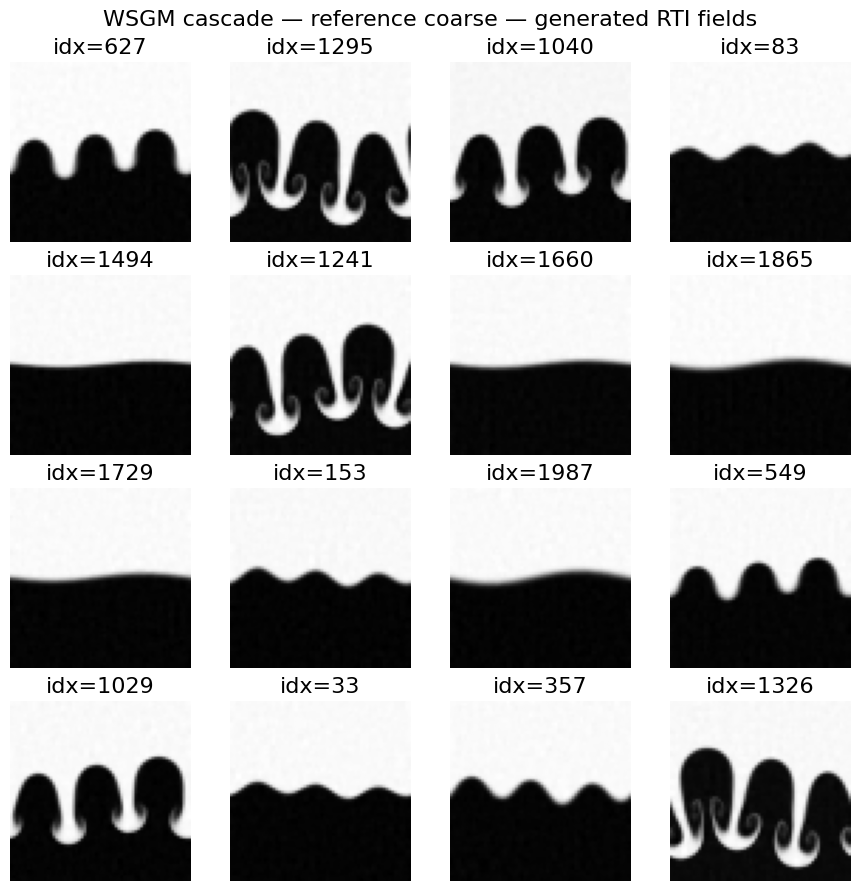
\includegraphics[
            width=\textwidth,
            height=\textwidth
        ]{figures/ch5/wsgm_reference_coarse_grid.png}
        \caption{WSGM with reference coarse coefficient, $128$ reverse steps.}
        \label{fig:ch5_reference_coarse_grid}
    \end{subfigure}
    \hfill
    \begin{subfigure}[c]{0.32\textwidth}
        \centering
        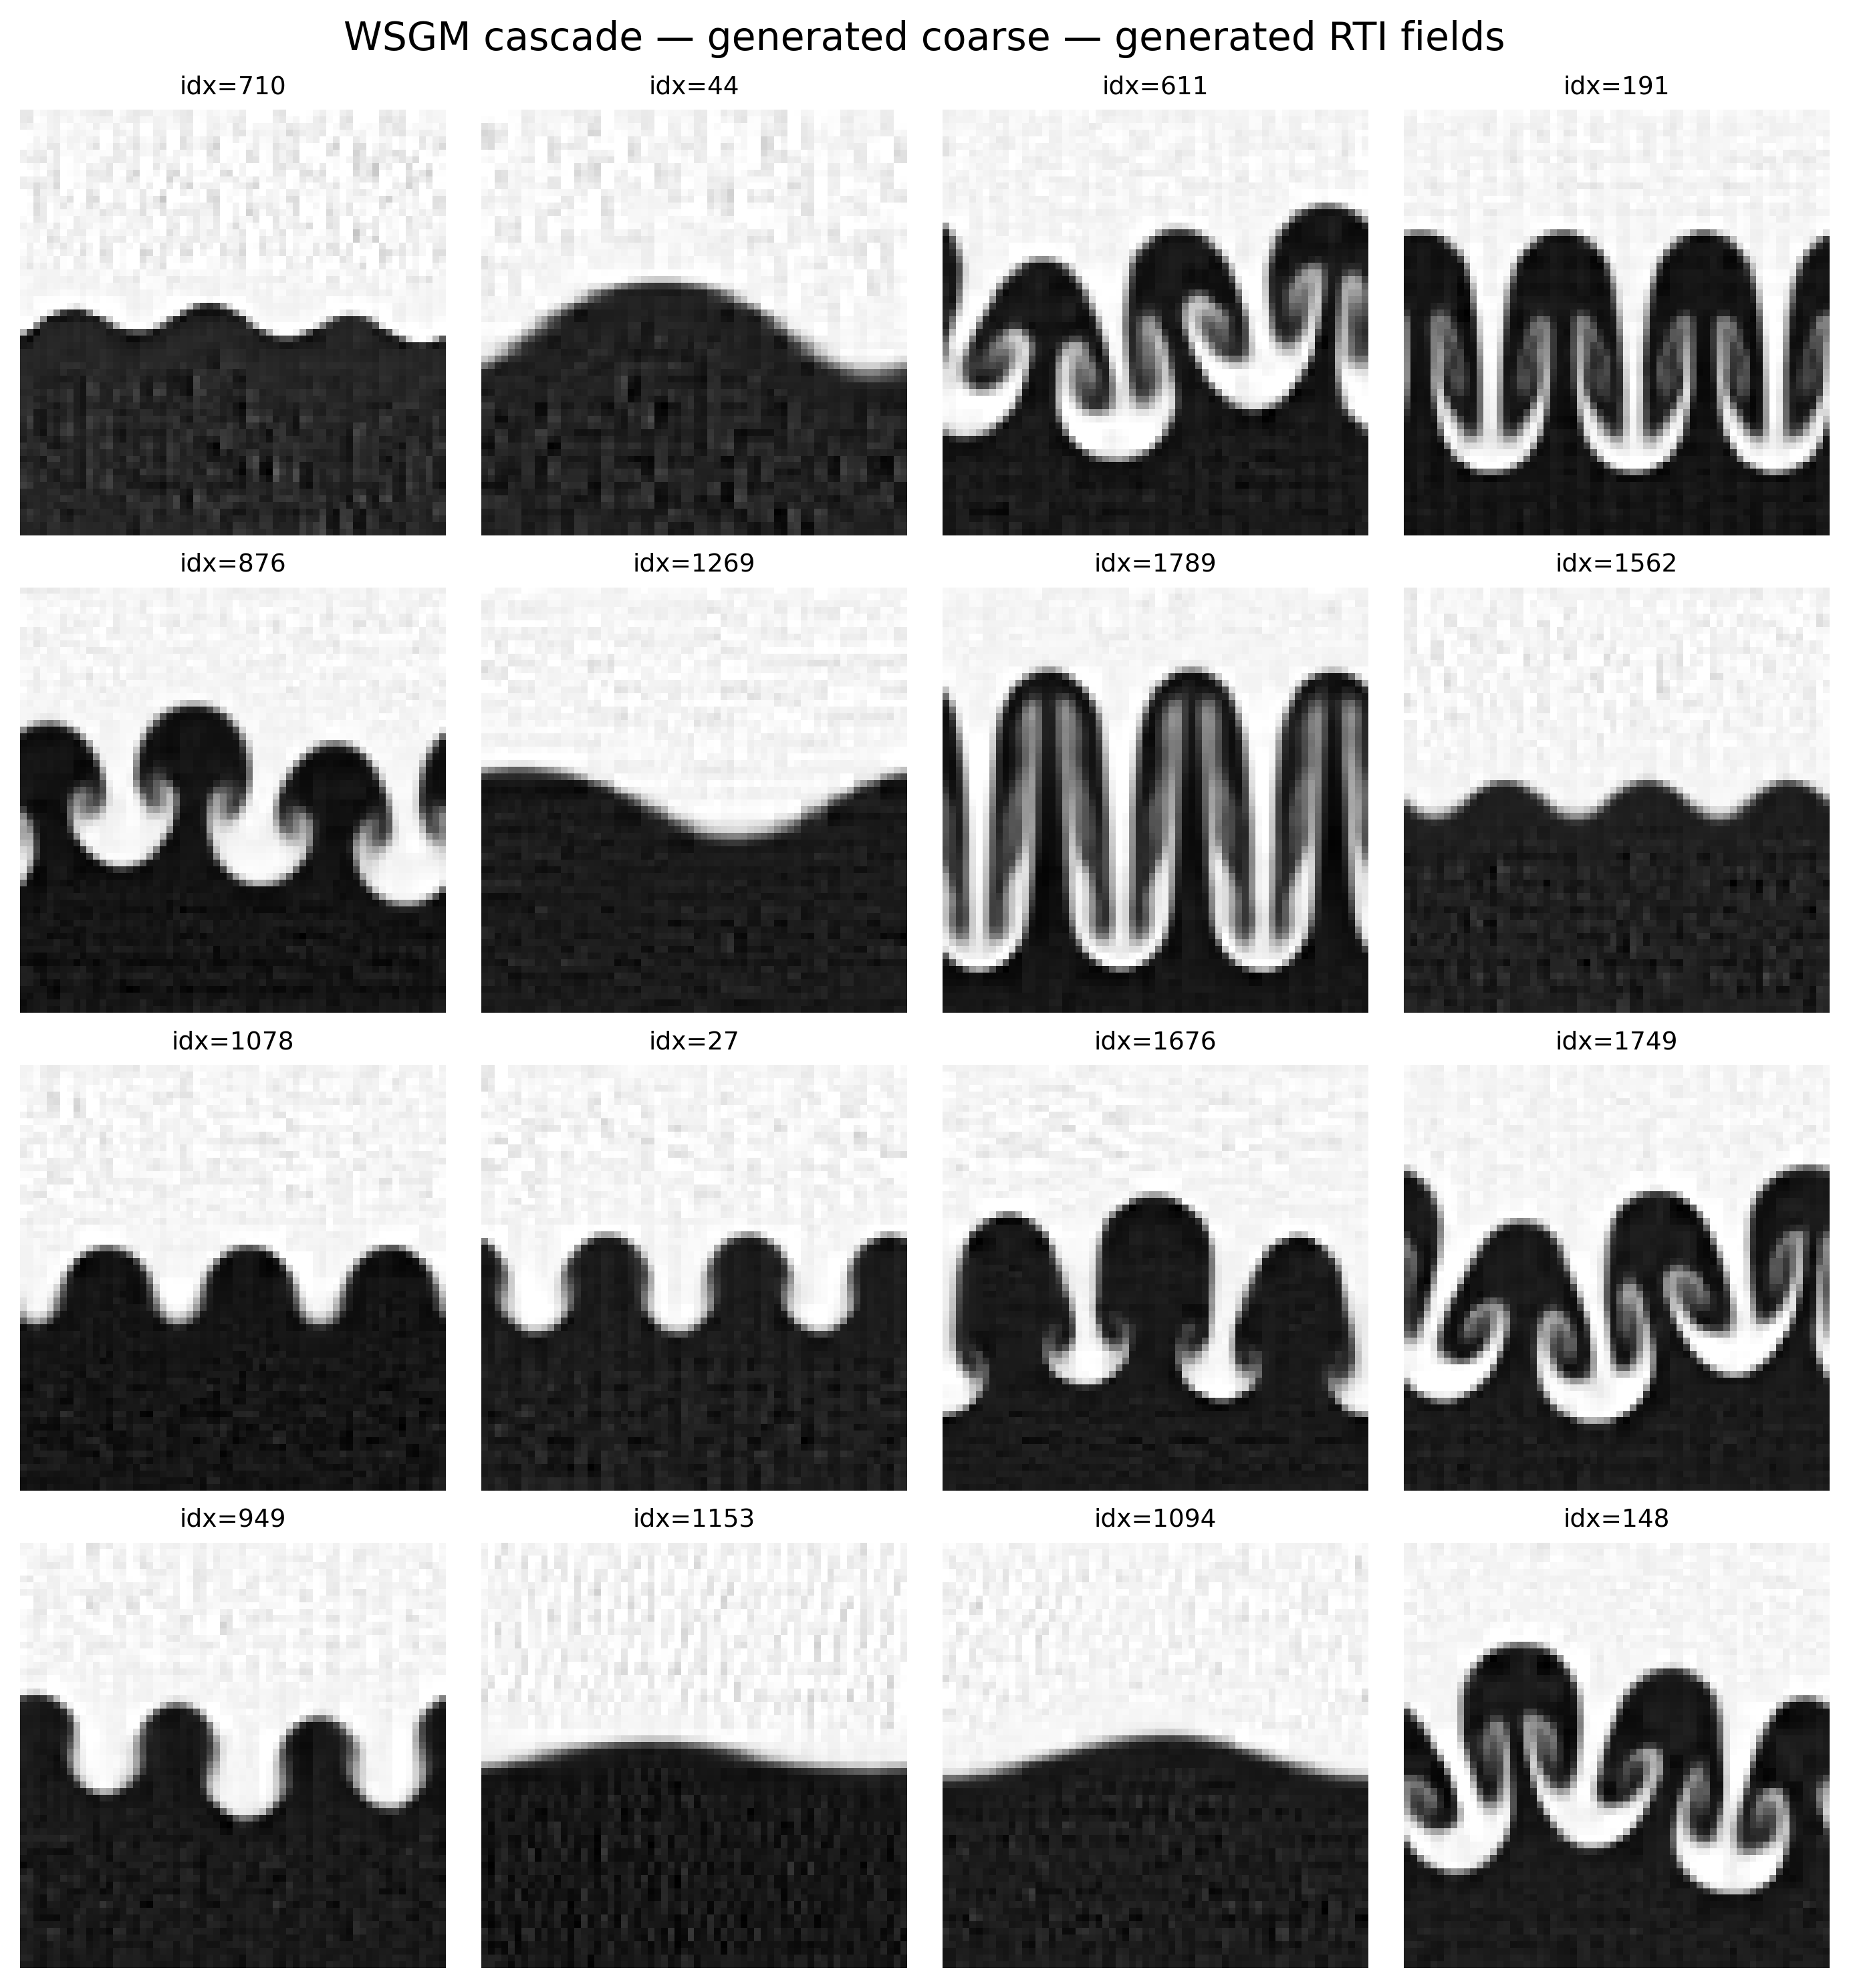
\includegraphics[
            width=\textwidth,
            height=\textwidth
        ]{figures/ch5/wsgm_generated_coarse_grid.png}
        \caption{WSGM with generated coarse coefficient, $128$ reverse steps.}
        \label{fig:ch5_generated_coarse_grid}
    \end{subfigure}

    \caption{Comparison between the SGM baseline (a), the WSGM with reference coarse coefficients (b), and the WSGM with generated coarse coefficients (c).}
    \label{fig:ch5_wsgm_field_comparison}
\end{figure}

To complement this visual inspection, Figure~\ref{fig:ch5_sgm_comparison_den}
compares the line-wise averaged density distributions. The fluctuation-energy
spectrum is not repeated for this wavelet comparison, because it did not add a
distinct qualitative ranking relative to the line-wise density statistic in the
present experiments. The mean vertical organization is therefore used as the
more compact physical diagnostic for comparing the three ensembles.

\begin{figure}[H]
    \centering

    \begin{subfigure}[c]{0.32\textwidth}
        \centering
        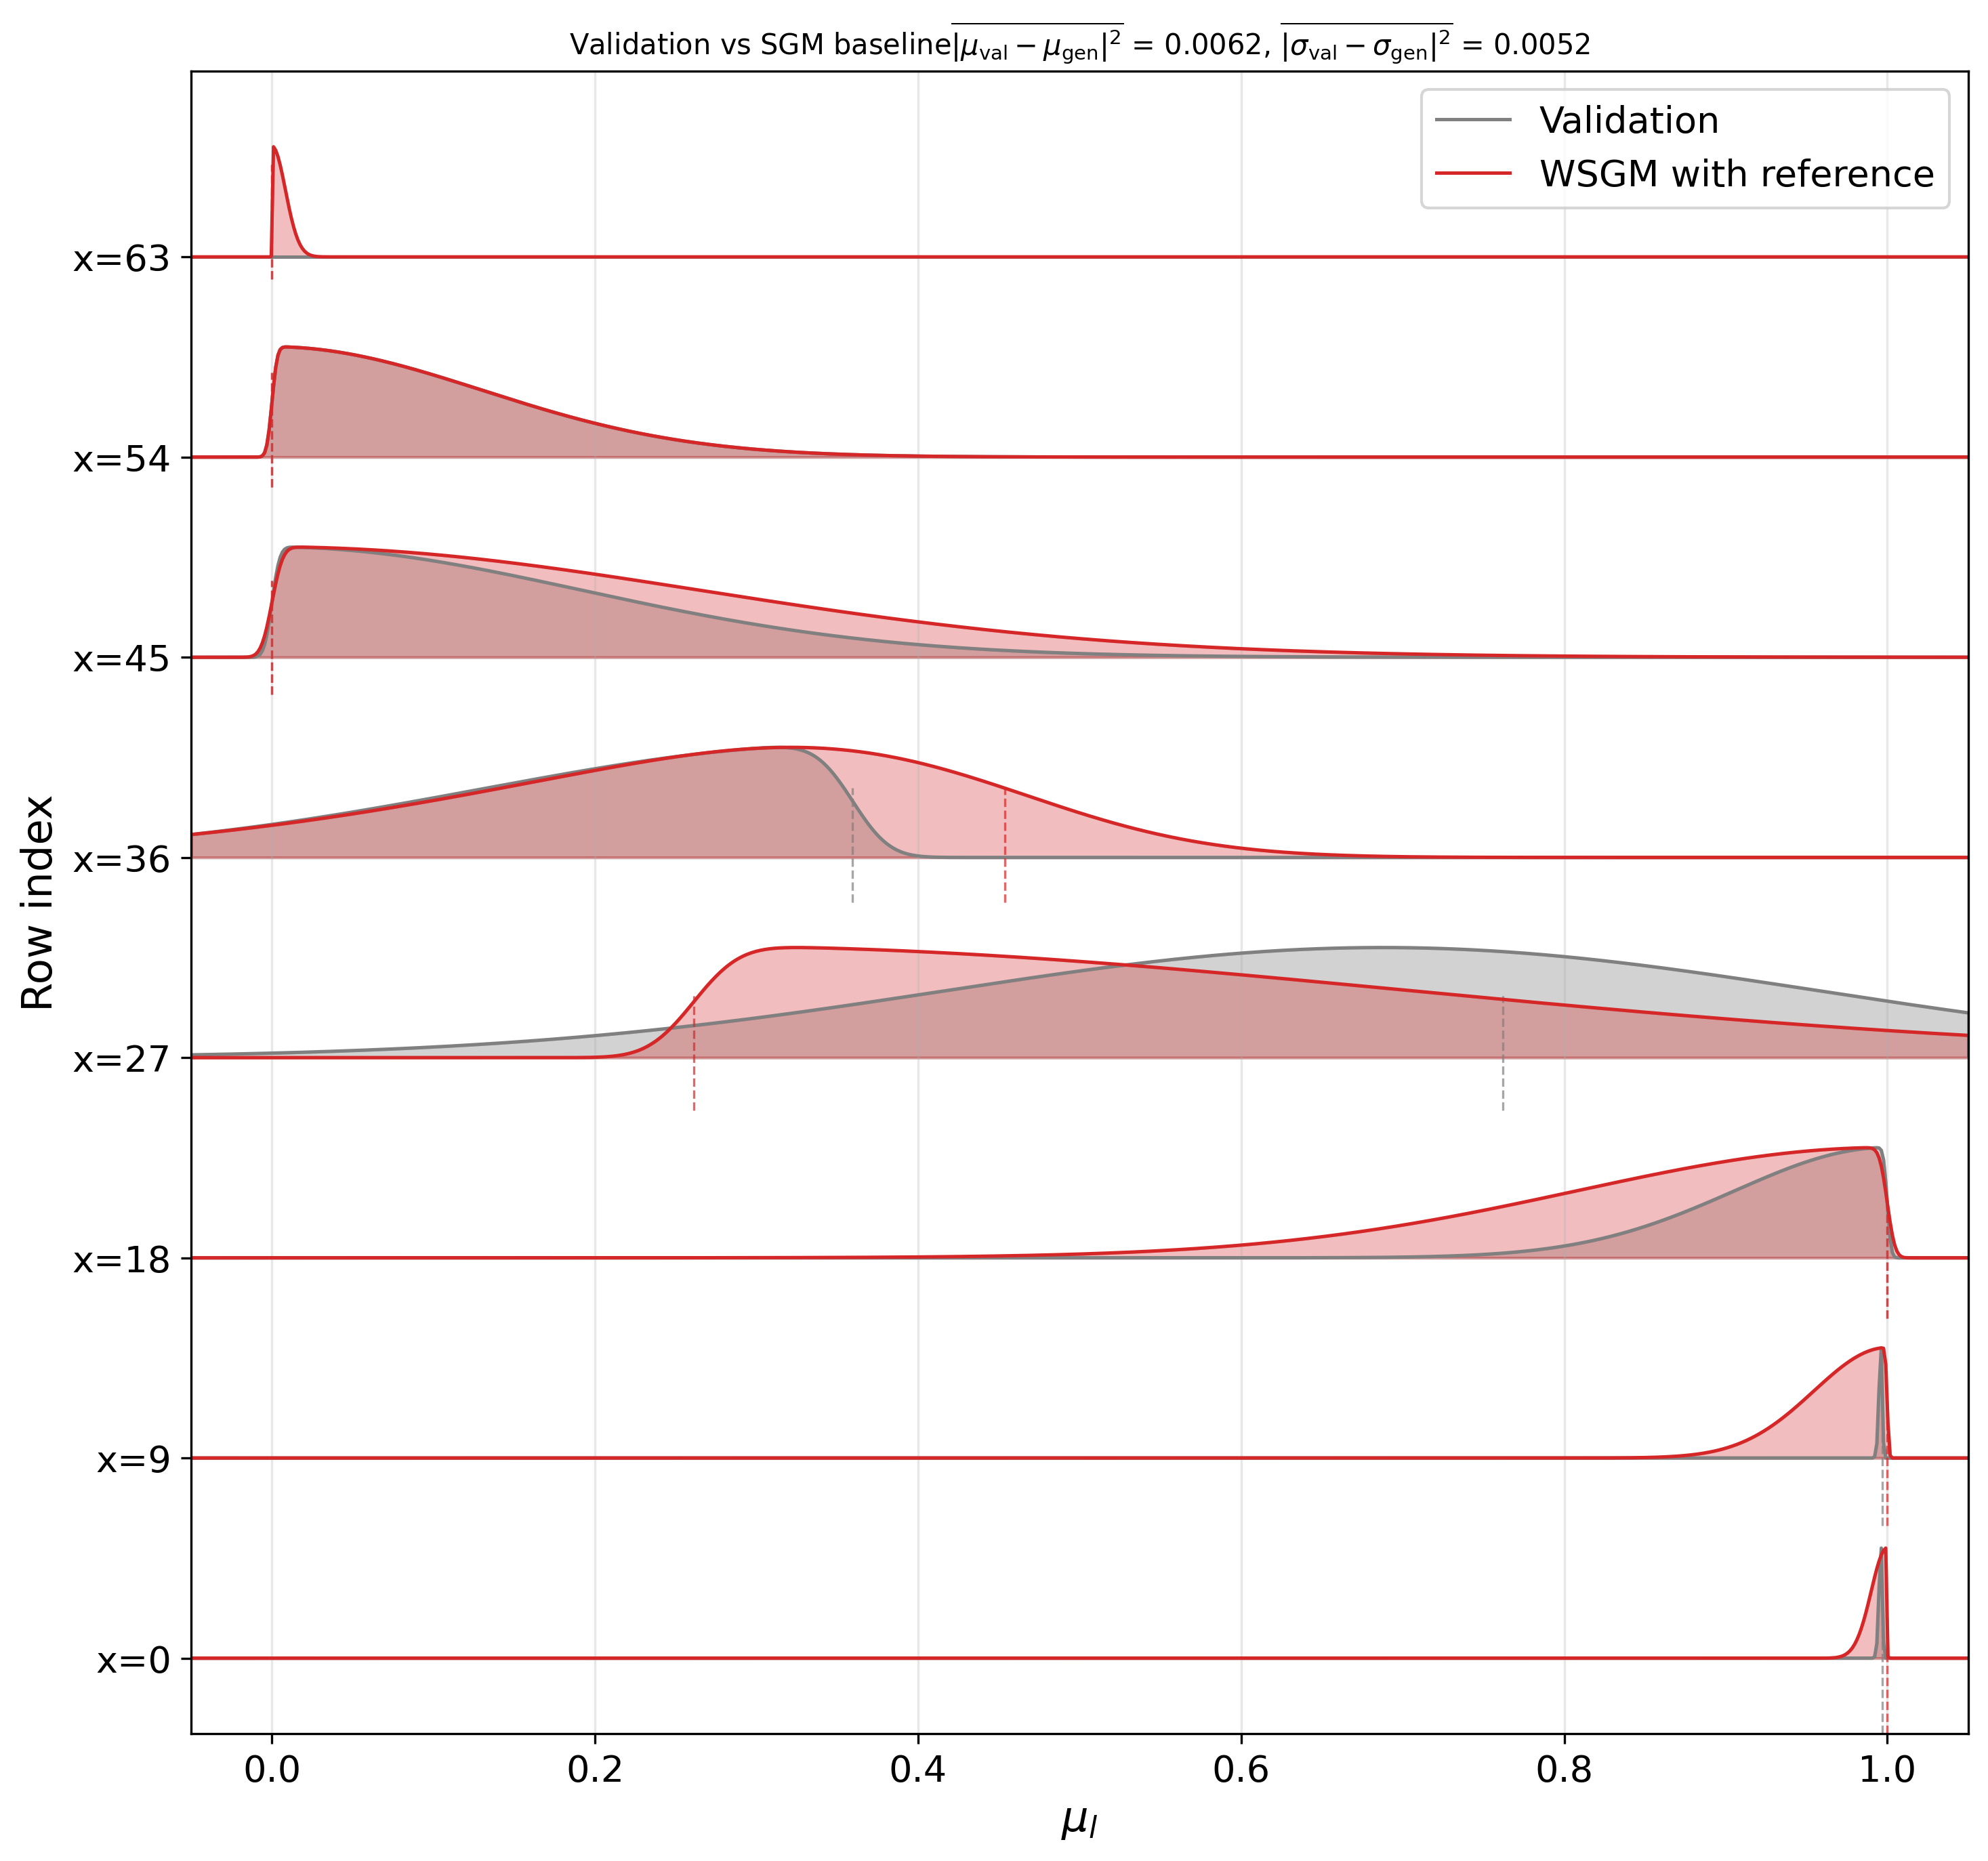
\includegraphics[
            width=\textwidth,
            height=\textwidth
        ]{figures/ch5/SGM_baseline_joyplot.png}
        \caption{SGM baseline with $128$ reverse steps.}
        \label{fig:ch5_den_original}
    \end{subfigure}
    \hfill
    \begin{subfigure}[c]{0.32\textwidth}
        \centering
        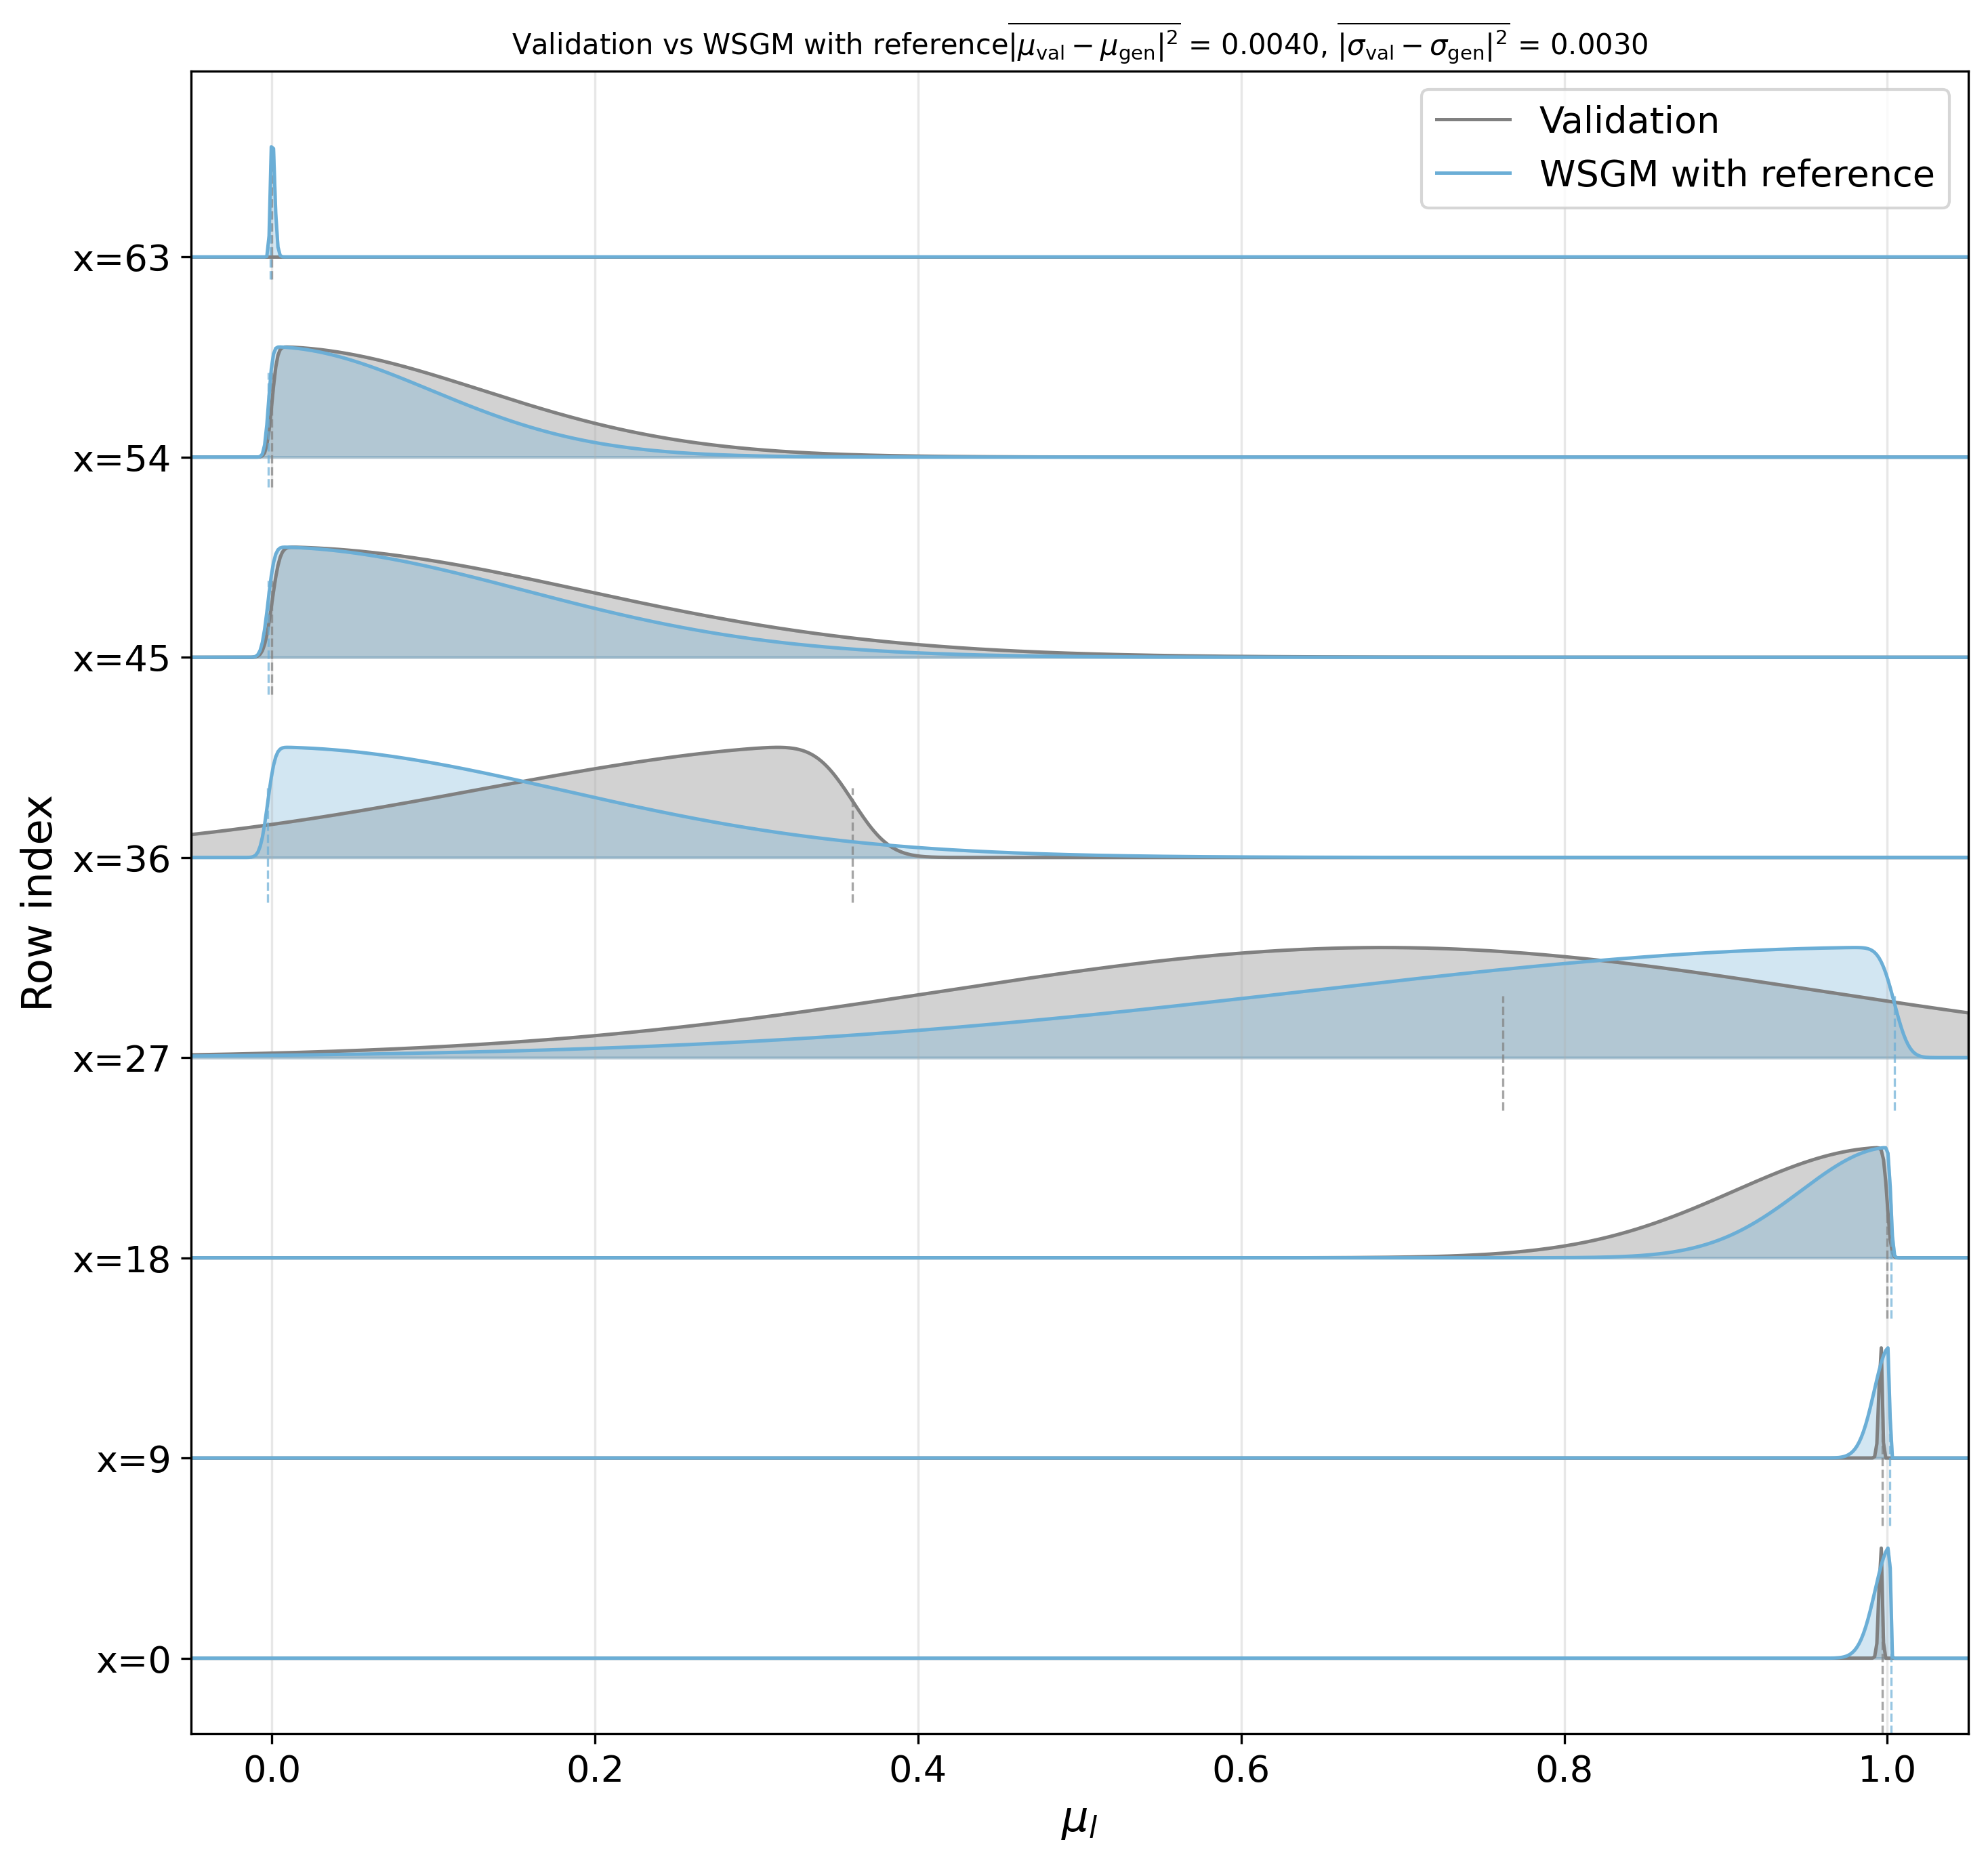
\includegraphics[
            width=\textwidth,
            height=\textwidth
        ]{figures/ch5/WSGM_ref_joyplot.png}
        \caption{WSGM with reference coarse coefficient, $128$ reverse steps.}
        \label{fig:ch5_den_reference_coarse_grid}
    \end{subfigure}
    \hfill
    \begin{subfigure}[c]{0.32\textwidth}
        \centering
        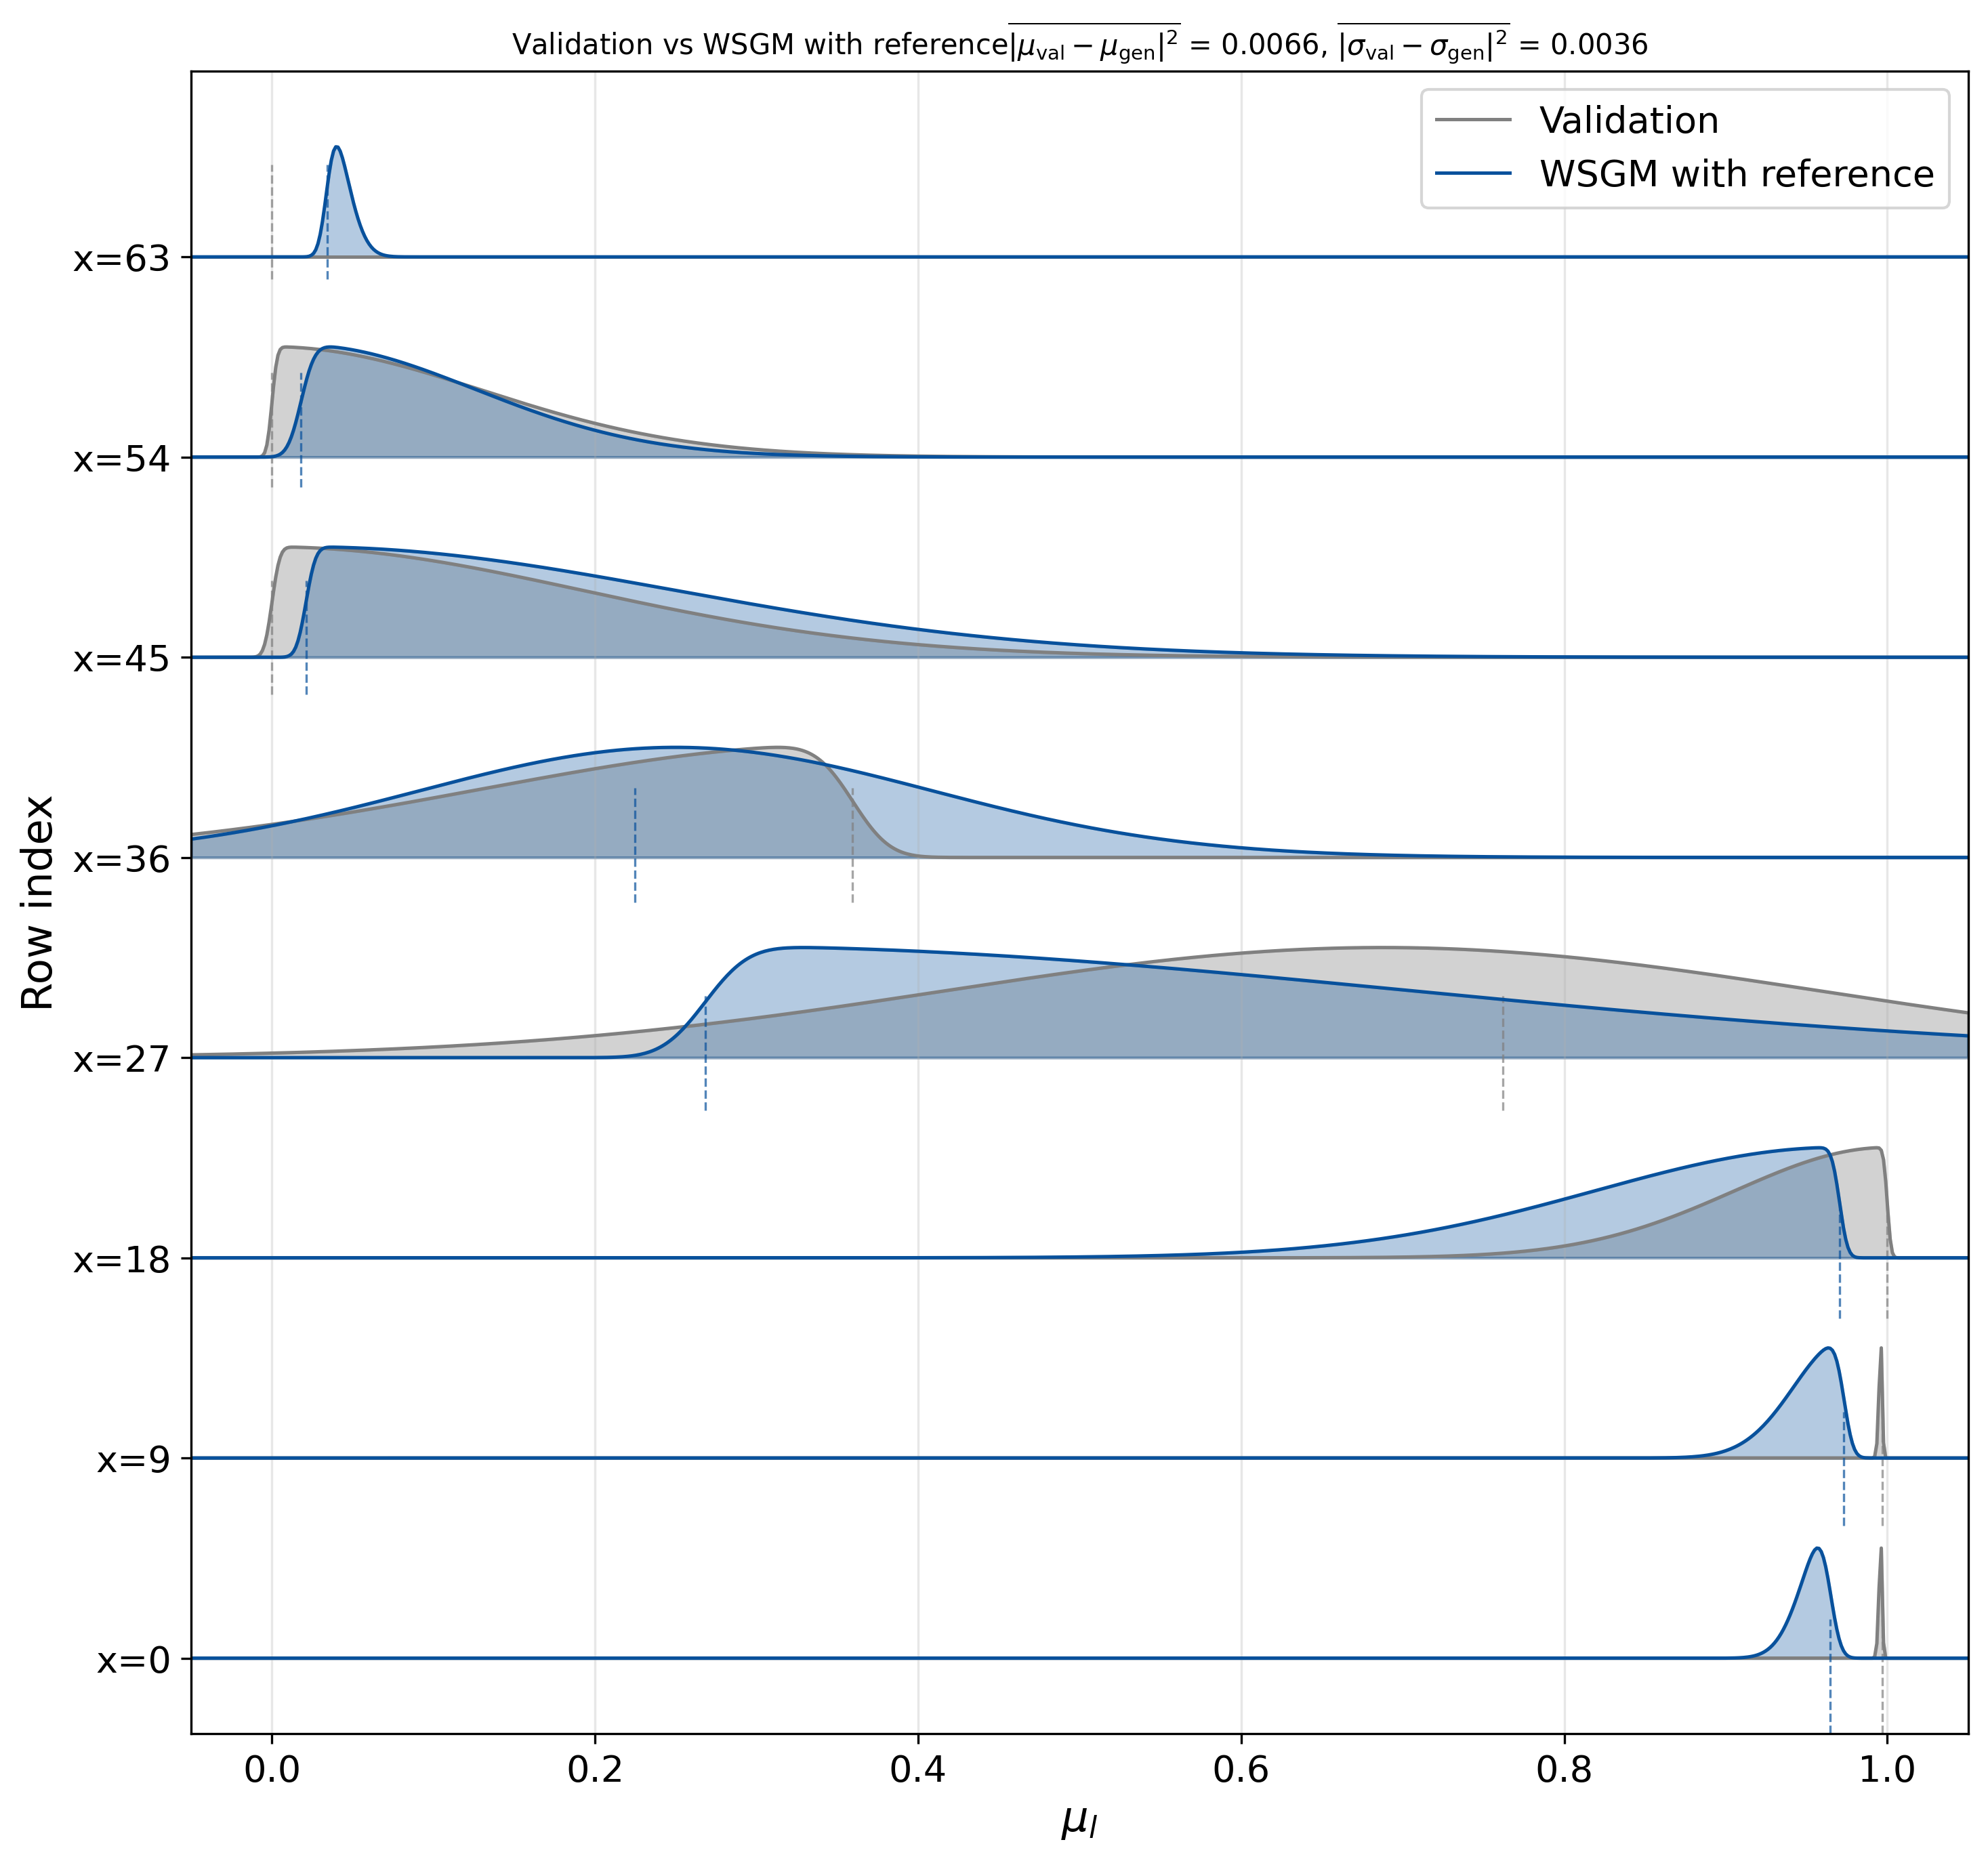
\includegraphics[
            width=\textwidth,
            height=\textwidth
        ]{figures/ch5/WSGM_gen_joyplot.png}
        \caption{WSGM with generated coarse coefficient, $128$ reverse steps.}
        \label{fig:ch5_den_generated_coarse_grid}
    \end{subfigure}

    \caption{Line-wise averaged density distributions for the SGM baseline (a), the WSGM with reference coarse coefficients (b), and the WSGM with generated coarse coefficients (c).}
    \label{fig:ch5_sgm_comparison_den}
\end{figure}

Figure~\ref{fig:ch5_phyfid_steps} separates the role of the wavelet detail
models from the role of the coarse diffusion model. The reference-coarse WSGM
should not be interpreted as a useful generative model by itself, since it uses
coarse information taken from a validation field. It is instead an oracle-coarse
ablation: it tests whether the wavelet cascade can generate accurate fine-scale
content when the coarse state is already physically consistent. The
generated-coarse curve then shows what remains when this favorable assumption is
removed.

\begin{figure}[H]
    \centering
    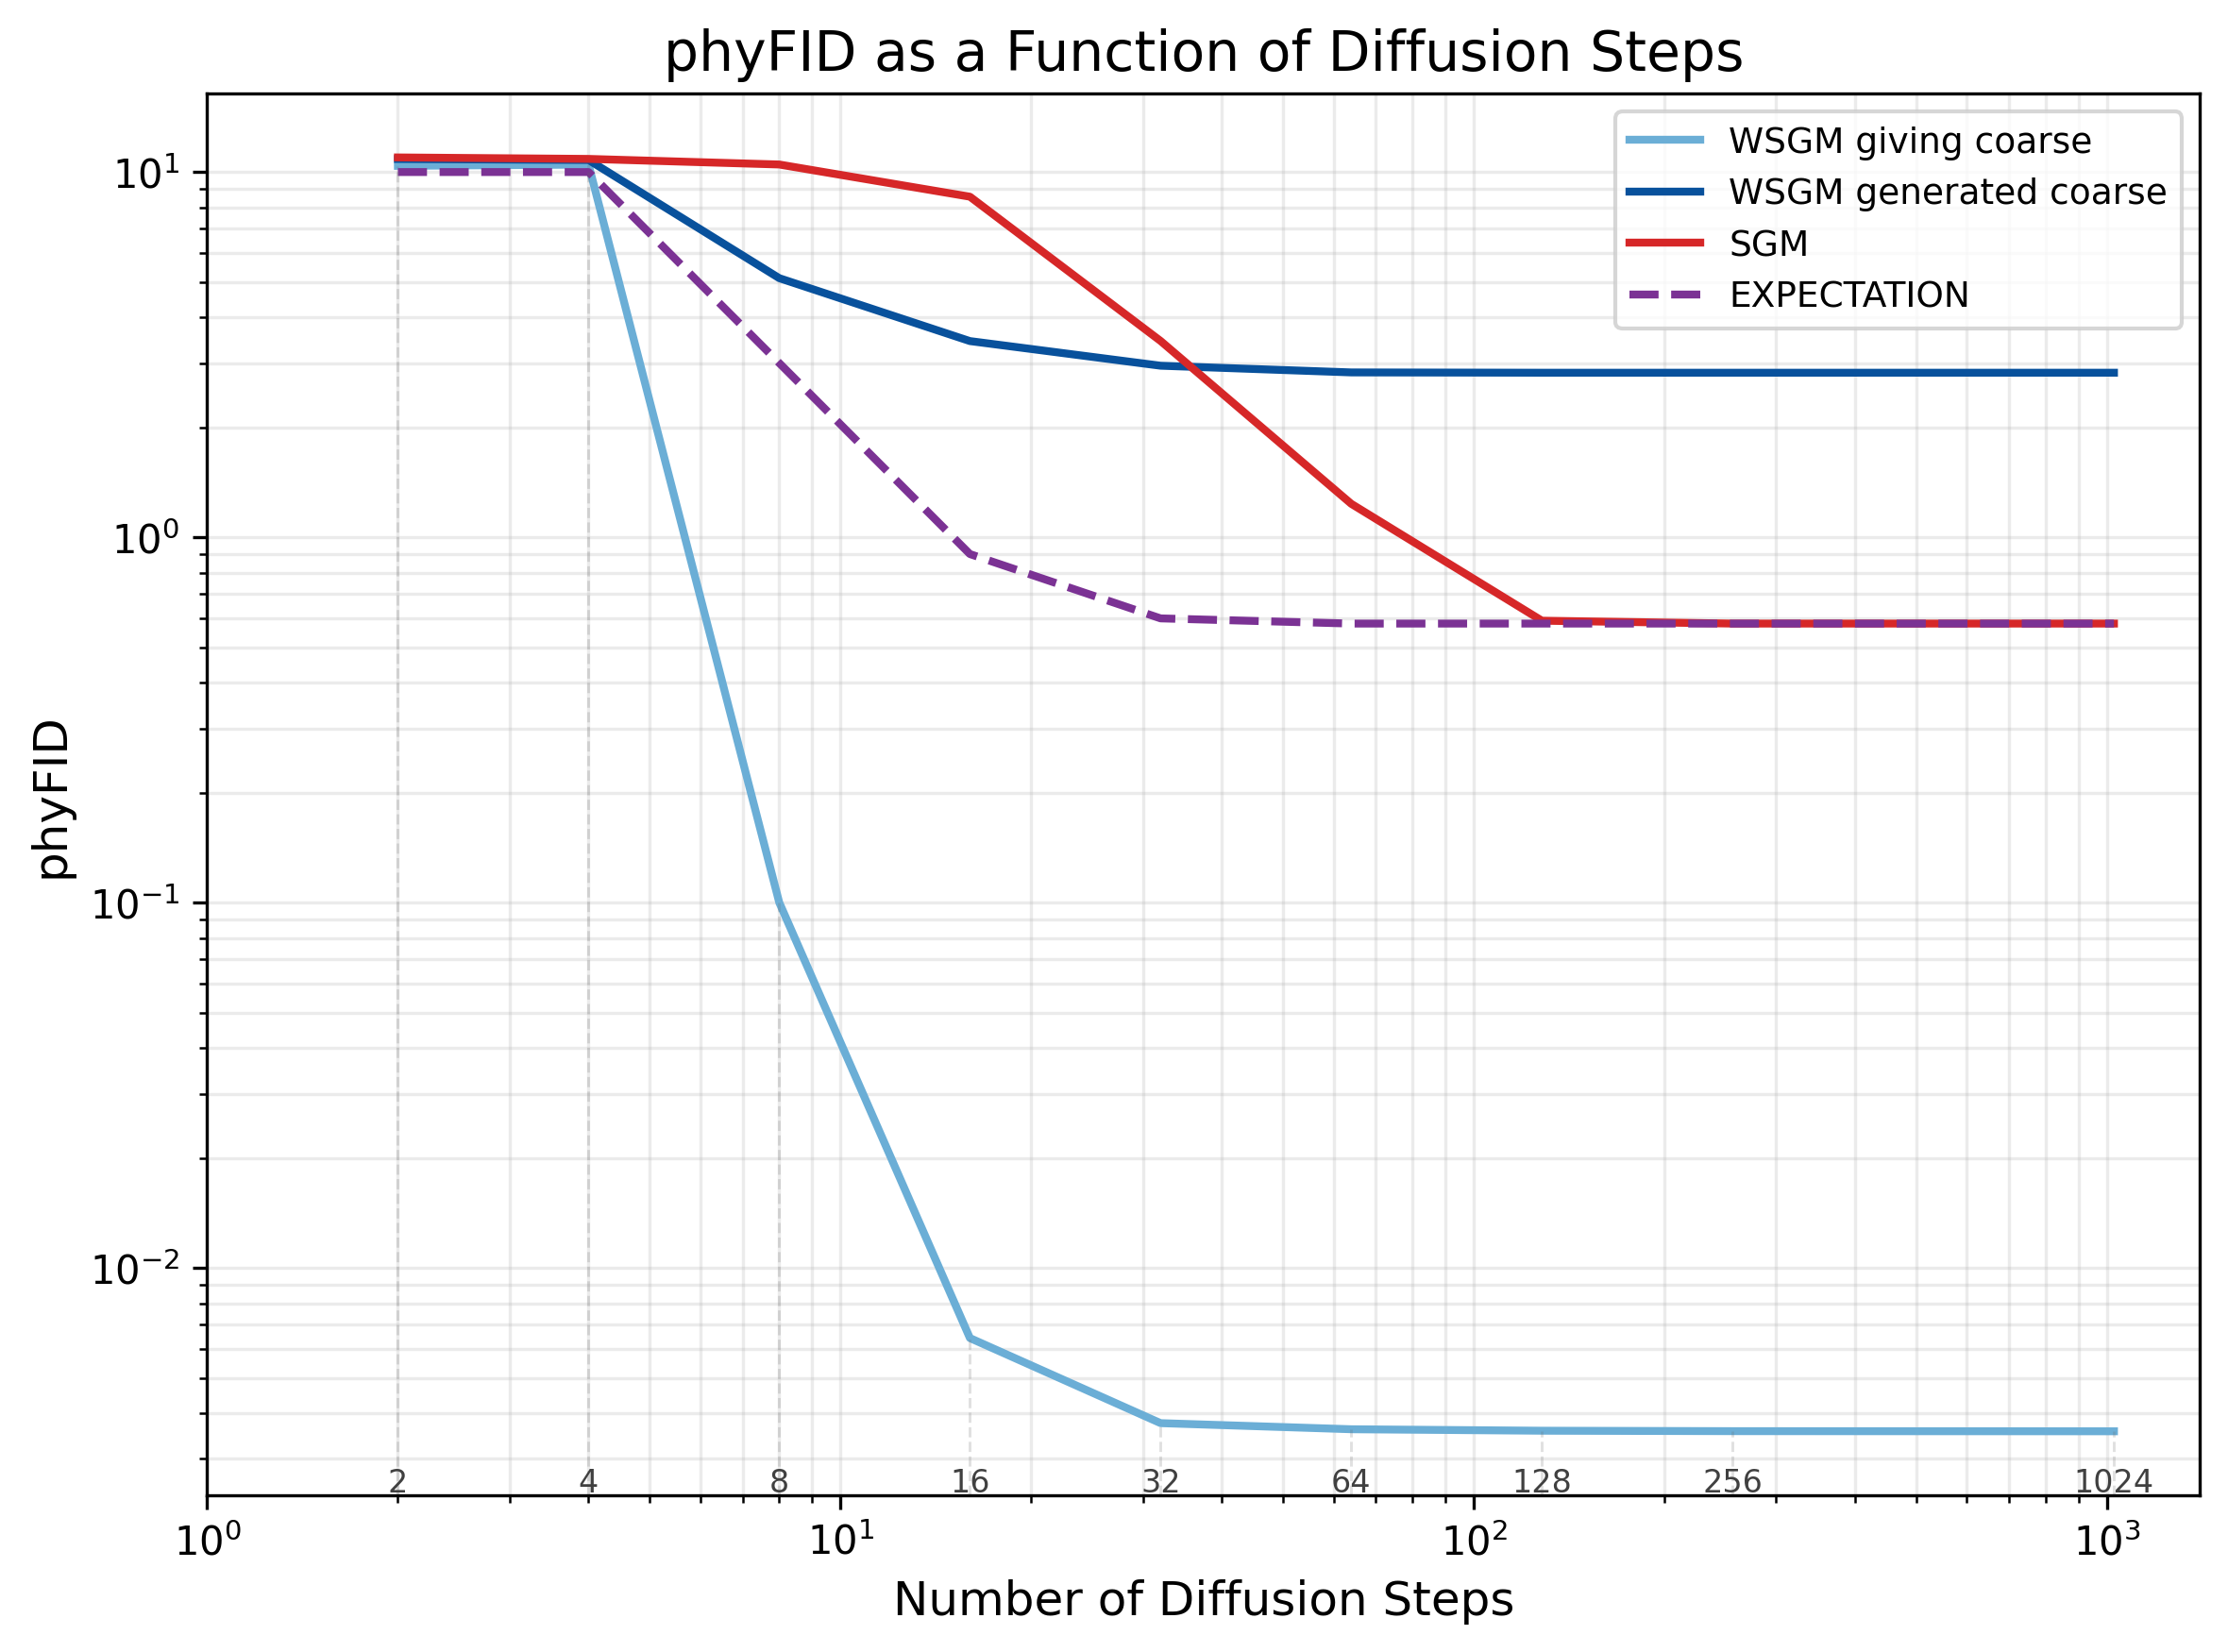
\includegraphics[width=0.90\textwidth]{figures/ch5/phyfid_vs_steps.png}
    \caption{PhyFID as a function of the number of reverse diffusion steps.
    The light-blue curve uses a reference coarse coefficient; the dark-blue
    curve corresponds to the unconditional wavelet cascade; the red curve is
    the direct SGM baseline. Lower is better.}
    \label{fig:ch5_phyfid_steps}
\end{figure}

With a reference coarse coefficient, PhyFID is $3.6\times10^{-3}$ at $64$
reverse steps and remains below $10^{-1}$ down to $8$ steps. This indicates
that the conditional wavelet detail models can work with a small number of
sampling steps, provided that the coarse coefficient has converged to the
correct distribution. In contrast, the fully generated cascade remains near
$2.83$ at $64$ steps and changes little when the number of steps is increased.
The current bottleneck is therefore the generated coarse coefficient, not the
conditional detail generation. The expectation curve summarizes the resulting
target: if the coarse model is improved, the WSGM cascade could recover the
quality of the direct SGM with fewer reverse steps.
